\documentclass[../thesis/thesis.tex]{subfiles}
\begin{document}

\chapter{Evaluation}
\label{chap:evaluation}

We believe it is possible to produce a \gls{vc} investment screening system that is efficient, robust and powerful. In Chapter~\ref{chap:design}, we described the development and structure of such a system. Our system identifies startup companies likely to receive additional funding or exit in a given forecast window. This system generates statistics and make recommendations that may assist \gls{vc} firms to efficiently and effectively screen investment candidates. In this chapter, we first outline our experimental design, and then we evaluate models developed by our system against criteria of efficiency, robustness and predictive power.

\begin{enumerate}

\item Efficiency. We evaluated efficiency by exploring the learning curves of our classification techniques and whether there is sufficient data to produce reliable statistics. In some cases, our system could use smaller training sets without significant reduction in predictive power. We also explored the time profile of our system. An indicative implementation of our system takes 46 hours to run.

\item Robustness. We evaluated robustness by evaluating our models against multiple reverse-engineered historical datasets and measuring their variance. We found variance evaluated across all metrics to be low, with more variance over shorter forecast windows. When we explored the feature weights for each model developed on different historical datasets, we found slight variance.

\item Predictive Power. We evaluated our system's predictive power across different forecast windows, for startups at different stages of their development lifecycle, and for different potential target outcomes. We find that our system's performance is positively related to longer forecast window (for 2-4 years), later developmental stage (e.g. Seed, Series A), and breadth of target outcome (e.g. Exit, Acquisition).

\end{enumerate}

\section{Experimental Design}

In the previous chapter, we produced a classification pipeline optimised with respect to its robustness over time. In our experimentation, we evaluated models produced by this pipeline against a held-out test dataset while varying a number of other factors. This evaluation process is depicted in Figure~\ref{fig:evaluation:pipeline_evaluation}. The pipeline is fit to a training dataset. The model is applied to a test feature vector to produce predictions. We score these predictions against truth values derived from the held-out test database (collected in April 2017). This process is performed multiple times to evaluate the three primary criteria derived from our literature review: efficiency, robustness and predictive power. The configuration of the system during our experiments is detailed in Appendix~\ref{appendix:experimental_config}.

\begin{figure}[!htb]
    \centering
    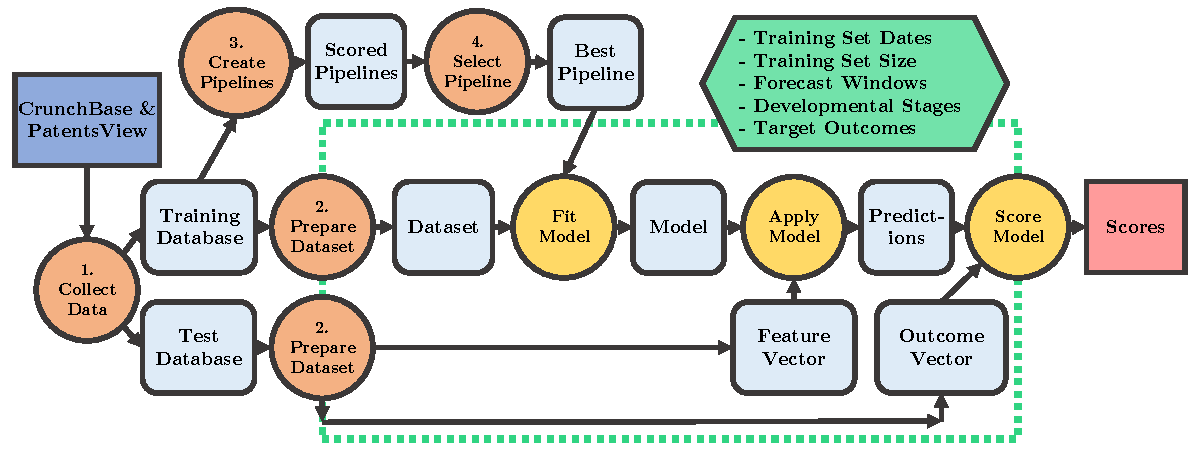
\includegraphics[width=\textwidth]{../figures/evaluation/flowchart_evaluation}
    \caption[Pipeline evaluation flowchart]{Pipeline evaluation overview. Legend: dark blue square = input, orange circle = system component, yellow circle = process, light blue rounded square = intermediate, red square = output, green hexagon: iterative process / search space.}
    \label{fig:evaluation:pipeline_evaluation}
\end{figure}

\subsection{Baseline Analysis}

Before we evaluated our system, we performed preliminary analyses to determine the baseline trends and distributions of company outcomes in our database.

First, we looked at company outcomes by forecast window. We applied the same system of reverse-engineering time slices that we used in previous experiments on robustness, but this time we varied the time difference between the slice that provides our features and the slice that provides our outcome. We combined pair-wise datasets of each year from 2012-2016 inclusive and explored the proportion of companies that raised additional funding or exited.

Figure~\ref{fig:evaluation:outcome_forecast_window} shows how company outcome varies with respect to the forecast window (time between the observed features and the measured outcome). We observe a positive relationship between length of forecast window and company outcome. Few companies appear to have exited or raised funds over a period of less than 2 years so we will focus our experimentation on forecast windows of 2-4 years.

\begin{figure}[!htb]
    \centering
    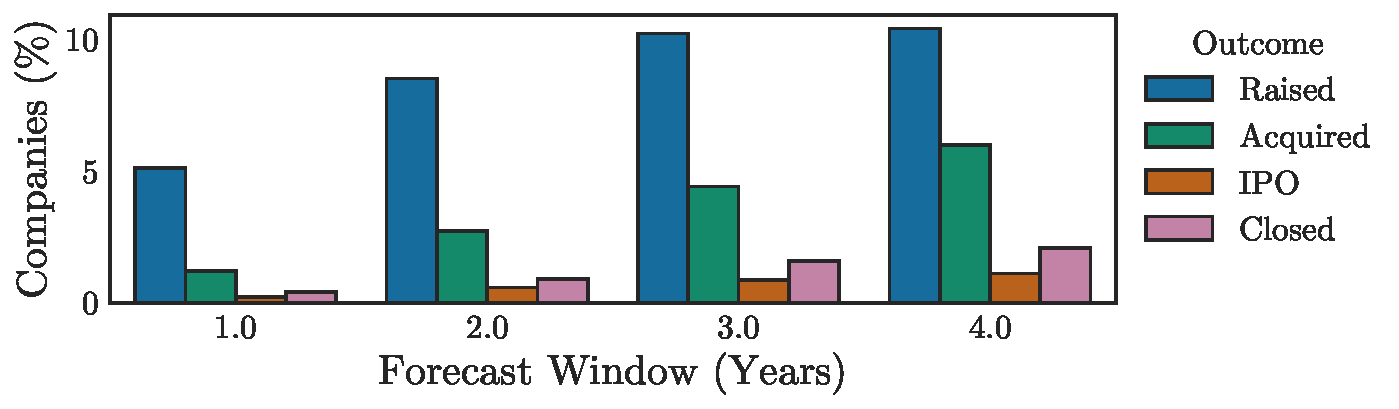
\includegraphics[width=\textwidth]{../figures/evaluation/outcomes_window}
    \caption[Outcomes by forecast window]{Outcomes by forecast window.}
    \label{fig:evaluation:outcome_forecast_window}
\end{figure}

We also looked at how company outcomes vary with respect to development stage, shown in Figure~\ref{fig:evaluation:outcome_stage}. We see a broad positive relationship between developmental stage and likelihood of further funding rounds and exits, which we would expect as at each stage there is higher market traction and scrutiny from investors. The variance between the outcomes of different developmental stages suggested that in our experimentation we should investigate how our system predicts each stage independently, as well as in aggregate.

\begin{figure}[!htb]
    \centering
    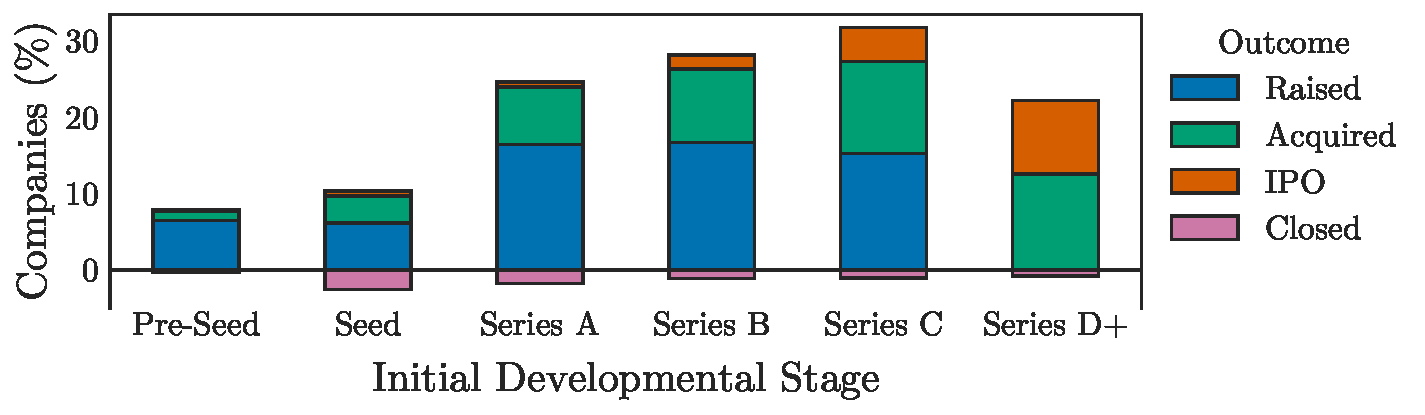
\includegraphics[width=\textwidth]{../figures/evaluation/outcomes_stage}
    \caption[Outcomes by developmental stage]{Outcomes by developmental stage.}
    \label{fig:evaluation:outcome_stage}
\end{figure}

\subsection{Evaluation Metrics}

While Area under the \gls{pr} Curve was used to guide the development of our system during pipeline optimisation, in evaluation of our system's performance we primarily use F1 Scores. An F1 score is the harmonic mean of recall and precision at points on the \gls{pr} curve. In this sense, the \gls{auc} measure provides an overall evaluation of a classification system, whereas the F1 Score evaluates a set of predictions. For investment screening, we're more sensitive to classification performance for the positive class (companies that have been successful in raising further funding or achieving an exit), so thereafter, when we refer to F1 Score, we refer to the F1 Score for this class alone. We also present \gls{mcc} in some of our analyses. \Gls{mcc} is a measure of the correlation between the observed and predicted binary classifications. It should produce similar results to a macro-averaged F1 Score, incorporating the performance of both classes.

\section{Efficiency}

The \gls{vc} industry requires more efficient forms of investment analysis, particularly in surfacing and screening. These processes are currently performed through referral, Google search, industry papers and manual search of startup databases. By its nature, our automated system should be more efficient than these methods. In this section, we assess how efficient our system is -- in terms of data consumed and time taken -- and look at whether we can further improve its efficiency.

\subsection{Dataset Size}

Learning curves allow us to evaluate how the bias and variance of a classification technique varies with respect to the amount of training data available. We investigated learning curves for our classification pipeline to determine whether smaller samples could achieve similar predictive power and reduce the system's computational demand. We applied 10-fold stratified cross-validation to split our dataset into 10 subsets of different sizes which we used to train the estimator and produce training and test scores for each subset size. The rate of convergence of our training and cross-validation curves implies whether our classification pipeline is over- or under-fitting our data for various sizes allowing us to select an optimal sample size.

Figure~\ref{fig:evaluation:learning_window} shows the learning curves for forecast windows of 2-4 years. The maximum number of training examples is negatively related to the length of the forecast window because newer datasets have more examples. For a forecast window of 4 years the curves have converged, whereas for shorter forecast windows there still seems to be some benefit to additional training examples. Much of the testing score improvement comes in the first 20,000 training examples, which suggests this pipeline is approaching optimal performance.

\begin{figure}[!htb]
    \centering
    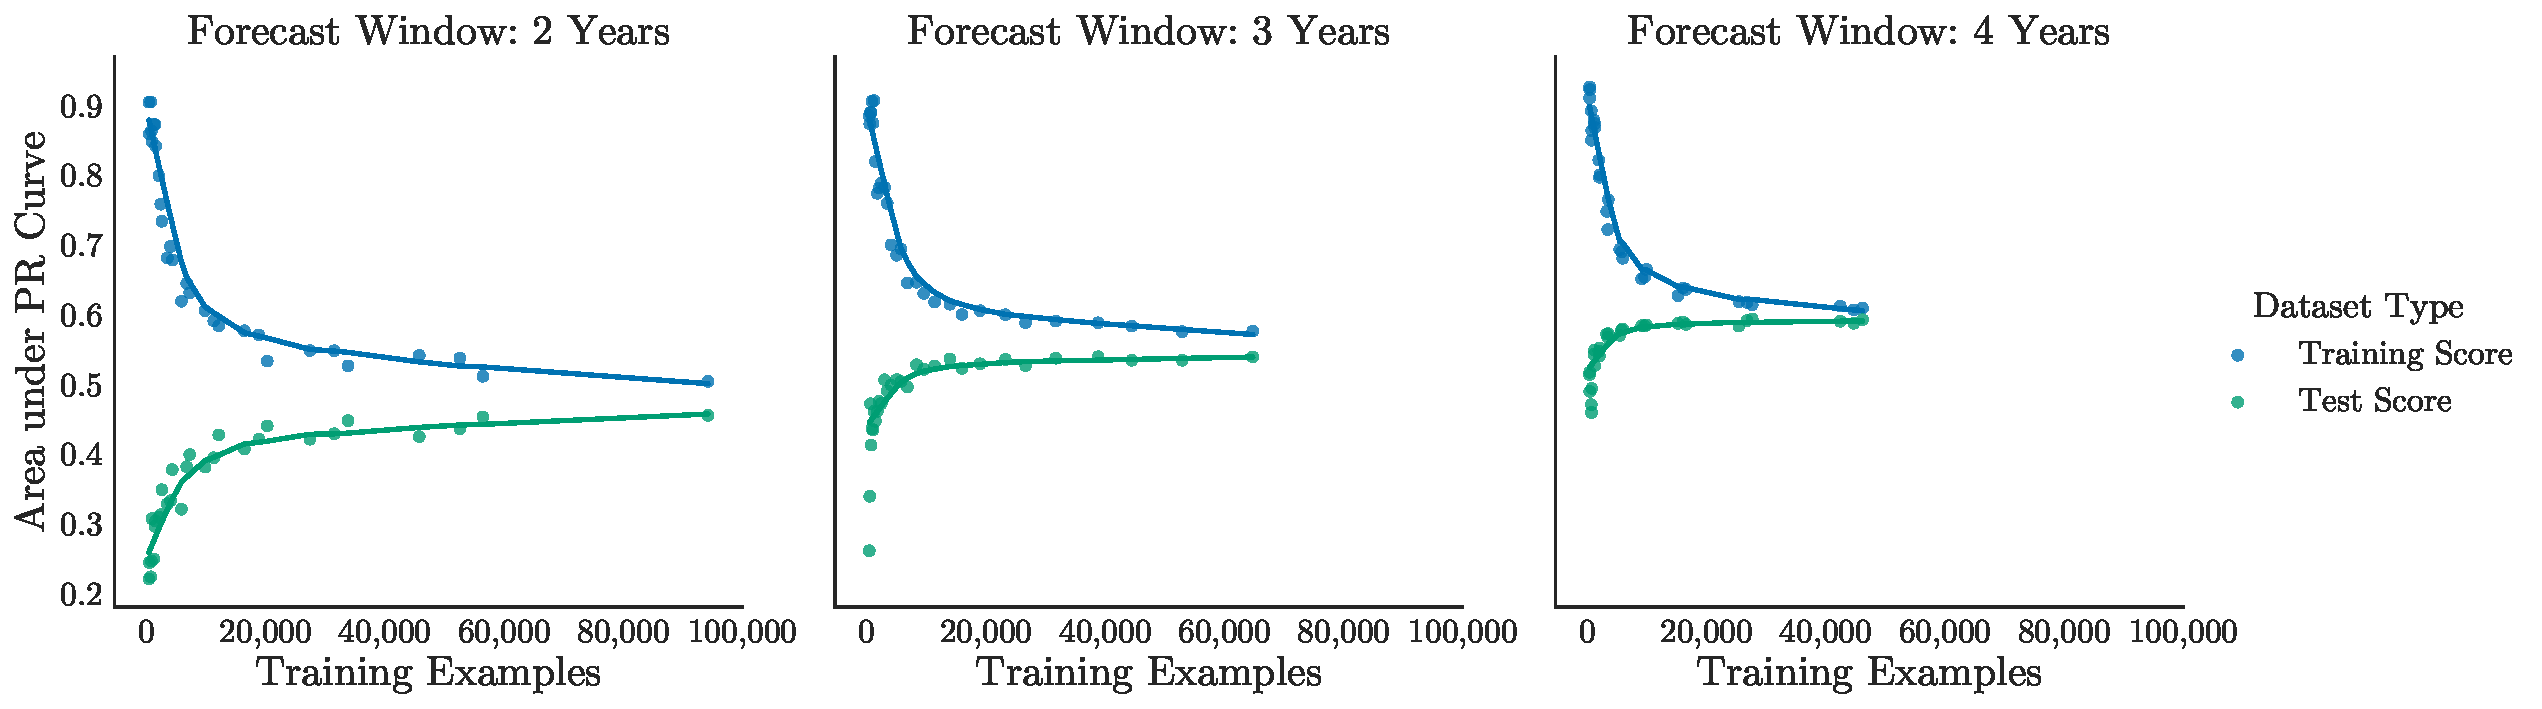
\includegraphics[width=\textwidth]{../figures/evaluation/learning_curves_window}
    \caption[Learning curves by forecast window]{Learning curves by forecast window.}
    \label{fig:evaluation:learning_window}
\end{figure}

%TODO - Learning curve by stage

\begin{figure}[!htb]
    \centering
    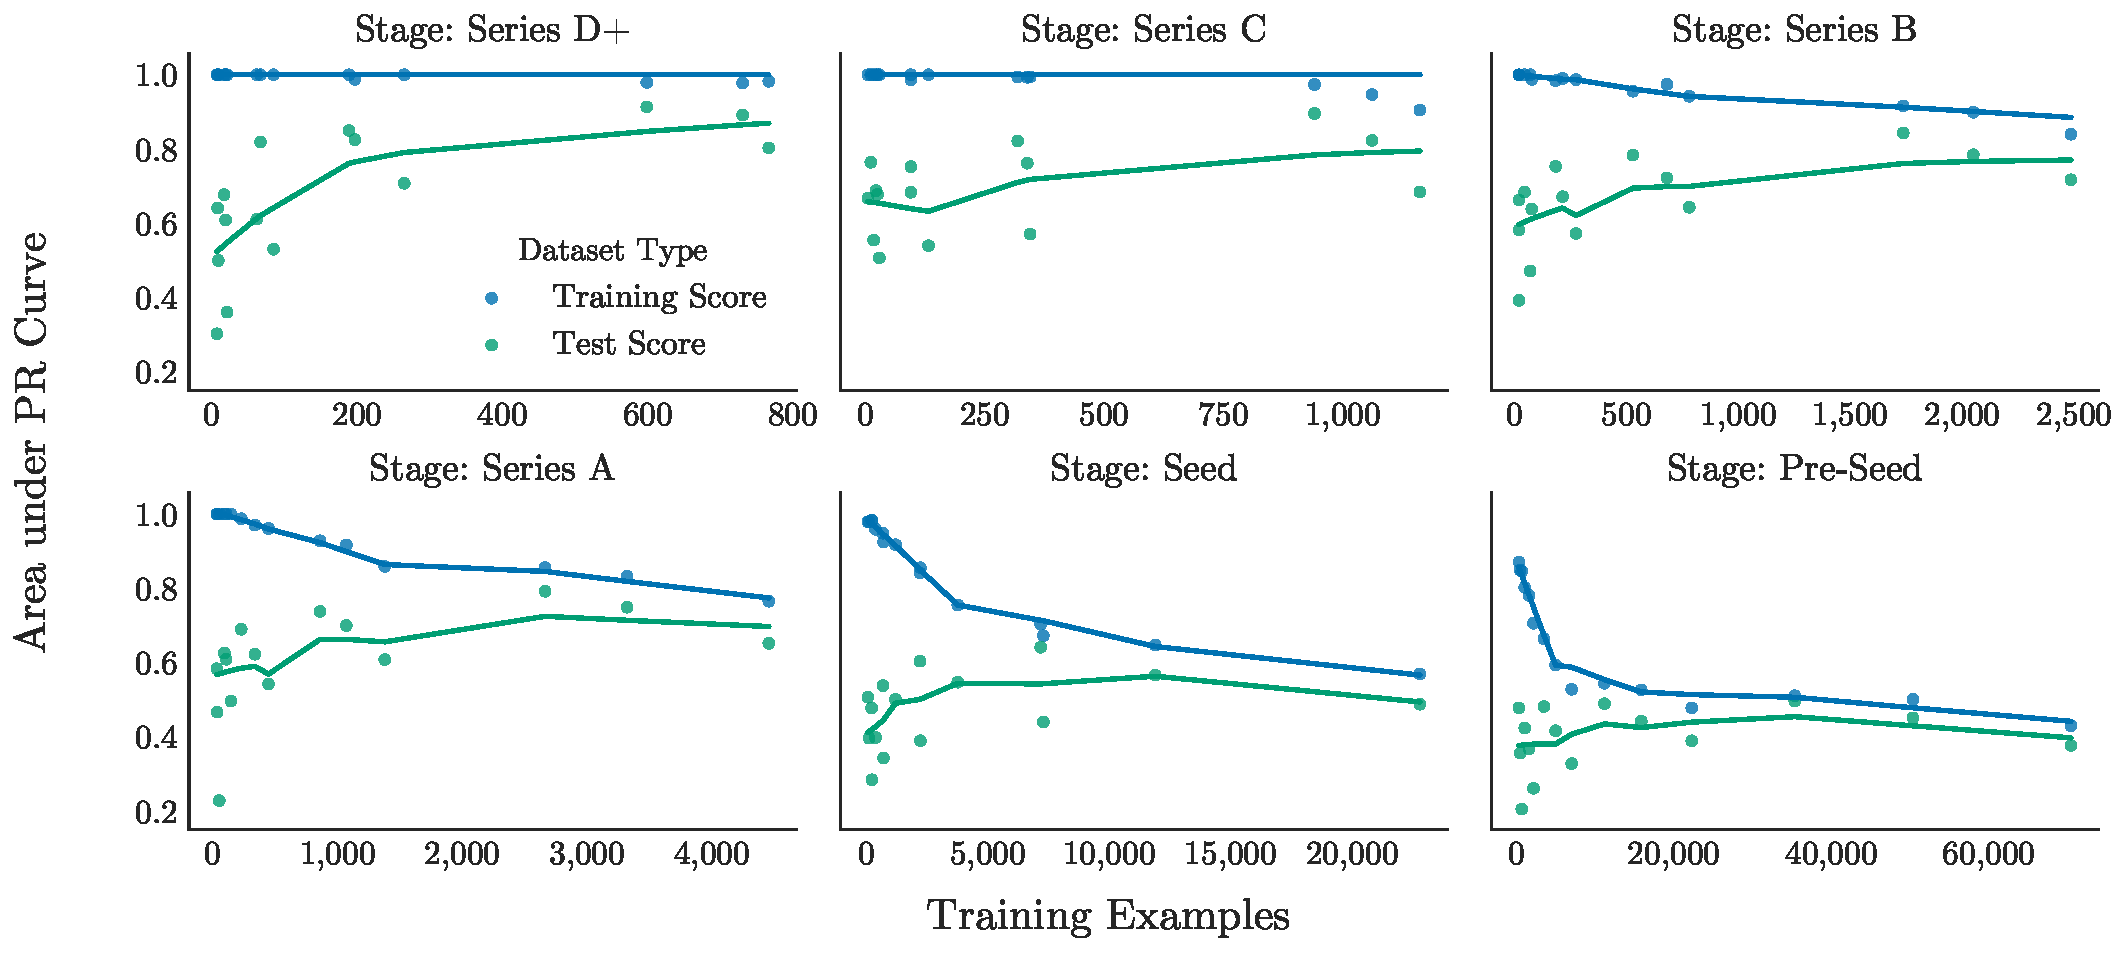
\includegraphics[width=\textwidth]{../figures/evaluation/learning_curves_stage}
    \caption[Learning curves by developmental stage]{Learning curves by developmental stage.}
    \label{fig:evaluation:learning_stage}
\end{figure}

The plots in Figure~\ref{fig:evaluation:learning_window} are evaluated against our base target outcome, which we term ``Extra Stage'' (i.e. whether a company raises an additional funding round, is aquired or has an \gls{ipo}). When our learning curves are split by components of this target outcome, we see that the efficiency of our system varies, as shown in Figure~\ref{fig:evaluation:learning_outcome_window}. We observe that predicting whether a company raises an extra round is the least data-intensive outcome, as it converges even over a forecast window of 2 years. In comparison, predicting company exits does not converge, even over a forecast window of 4 years. Our model has most difficulty predicting \gls{ipo} exits, which are rare events in our dataset.

\begin{figure}[!htb]
    \centering
    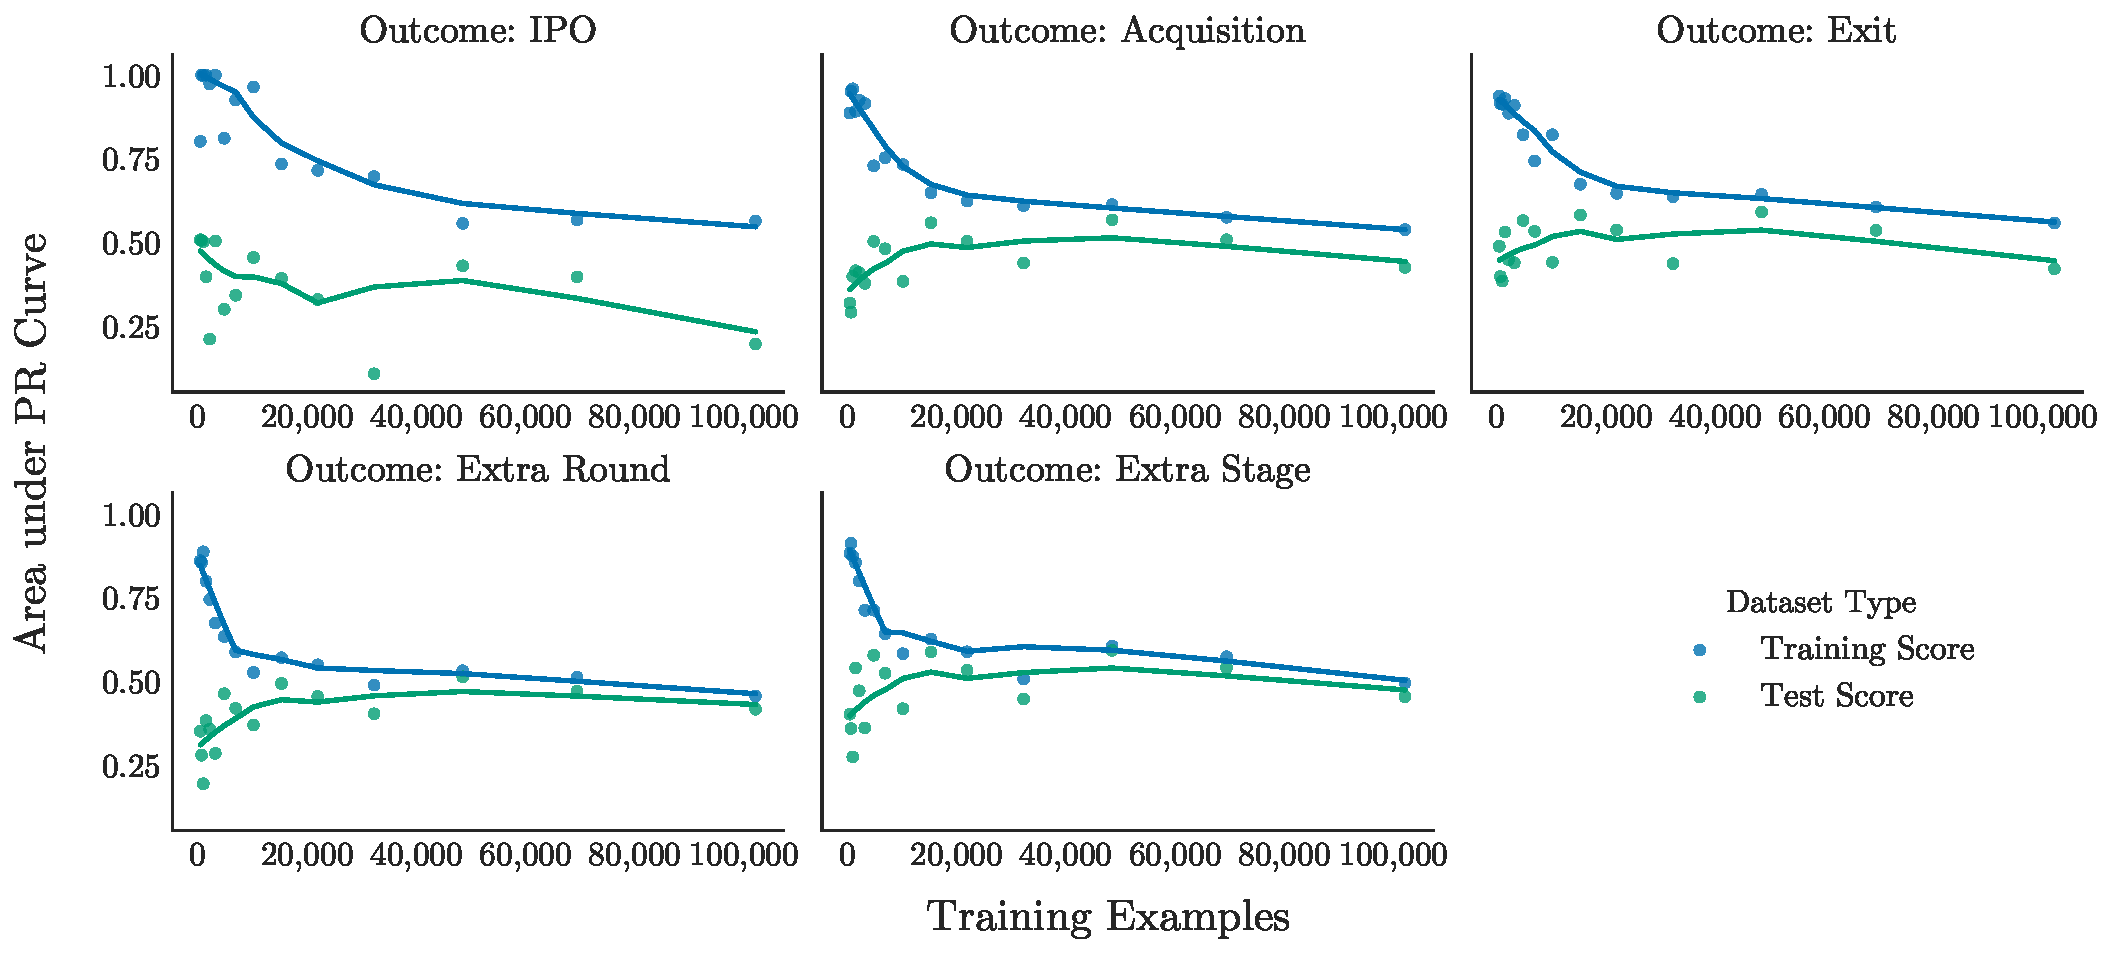
\includegraphics[width=\textwidth]{../figures/evaluation/learning_curves_outcome}
    \caption[Learning curves by target outcome]{Learning curves by target outcome (column) and forecast window (row).}
    \label{fig:evaluation:learning_outcome_window}
\end{figure}

\subsection{Time Profile}

Unlike other forms of finance, like equity or derivatives trading, \gls{vc} operates on a much longer timeframe -- deals close over weeks, rather than minutes. This has two key disadvantages: \gls{vc} firms have higher management costs because they spend more time screening investments and startup founders waste precious time negotiating with investors when they could be building their businesses. Automated systems could decrease the time taken to generate investment opportunities. We investigated the time profile of our system to determine whether it is practical for use in the \gls{vc} industry.

An indicative time profile of the system is shown in Table~\ref{tab:evaluation:time_profile}. At the highest-level, this configuration of the program takes 46 hours to complete on a modern desktop PC. When we further break this time down by system component, the vast majority of time (84.8\%) is taken up by the initial pipeline creation component. This time is due to the pipeline optimisation process - the model is fit and scored over 500 times on different classification algorithms and parameters. Scoring takes a long time because, in this case, it also involves generating learning curves for reporting, which is another cross-validated process.

\begin{table}[!htb]
    \centering
    \scalebox{0.9}{\newcommand{\sub}[1]{\hspace{1em}#1}

\begin{tabular}{lrrrrr} \toprule
Function & Cycle (s) & Cycles (N) & Time (s)   & Time (m) & Time (h) \\ \midrule
Generate Dataset (CV)             & 1,800 & 1 & 1,800 & 30 & 0.5 \\
\sub{Prepare Feature Dataset}     & 1,200 & 1 & 1,200 & 20 & 0.3 \\
\sub{Prepare Outcome Dataset}     & 180 & 1 & 180 & 3 & 0.1 \\
\sub{Merge Datasets}              & 360 & 1 & 360 & 6 & 0.1 \\
\sub{Finalise Dataset}            & 60 & 1 & 60 & 1 & 0.0 \\
Fit and Score Model\textsuperscript{1} & 265 & 525 & 139,125 & 2,319 & 38.6 \\
\sub{Fit Model}                   & 15 & 525 & 7,875 & 131 & 2.2 \\
\sub{Score Model}                 & 250 & 525 & 131,250 & 2,188 & 36.5 \\ \midrule
\multicolumn{3}{l}{Subtotal: Create Pipelines} & 140,925 & 2,349 & 39.1 \\ \midrule
Get Finalist Pipelines            & 5 & 1 & 5 & 0 & 0.0 \\
Generate Dataset (CV)             & 1,800 & 5 & 1,800 & 30 & 0.5 \\
Fit and Score Model\textsuperscript{2} & 265 & 75 & 19,875 & 331 & 5.5 \\
Select Best Pipeline              & 5 & 1 & 5 & 0 & 0.0 \\ \midrule
\multicolumn{3}{l}{Subtotal: Select Best Pipeline} & 21,685 & 361 & 6.0 \\ \midrule
Generate Dataset (Training)       & 1,800 & 1 & 1,800 & 30 & 0.5 \\
Generate Dataset (Test)           & 1,800 & 1 & 1,800 & 30 & 0.5 \\
Fit Model                         & 30 & 1 & 30 & 1 & 0.0 \\
Make Predictions                  & 5 & 1 & 5 & 0 & 0.0 \\ \midrule
\multicolumn{3}{l}{Subtotal: Fit and Make Predictions} & 3,635 & 61 & 1.0 \\ \midrule
\multicolumn{3}{l}{Total}        & 166,245 & 2,771 & 46.2 \\
\bottomrule \end{tabular}
}
    \caption[System time profile]{System time profile.}
    \label{tab:evaluation:time_profile}
\end{table}

\section{Robustness}

The \gls{vc} industry is concerned that predictive models trained on historical data will not predict future trends and activity. This  has been identified as a key barrier to the adoption of automated systems by the \gls{vc} industry \cite{stone2014}. Therefore, it is critical that our system is shown to be robust in its performance with respect to time so investors can rely on its predictions.

We generated three models from datasets created from our training database from each year of 2012-2014 for forecast windows of 2 years (i.e. [2012, 2014], [2013, 2015], and [2014, 2016]) and evaluated each model against a dataset created from our test database (i.e. [2015, 2017]). We expected that if the factors that predict startup investment success through time are consistent, we would observe little difference between the performance and characteristics of these models.

Figure~\ref{fig:evaluation:performance_slice} shows the standard deviations of models trained on dataset slices from different years, against key evaluation metrics. We grouped by forecast windows as later dataset slices cannot be tested with long forecast windows which would skew results along this dimension. Variance across metrics is low, with more variance over shorter forecast windows.

We explored the feature weights for each model in Figure~\ref{fig:evaluation:features_slice}. While there are some slight differences, the general trend is similar across all models. We will discuss the distribution of these feature weights in more detail in a following section.

\begin{figure}[!htb]
    \centering
    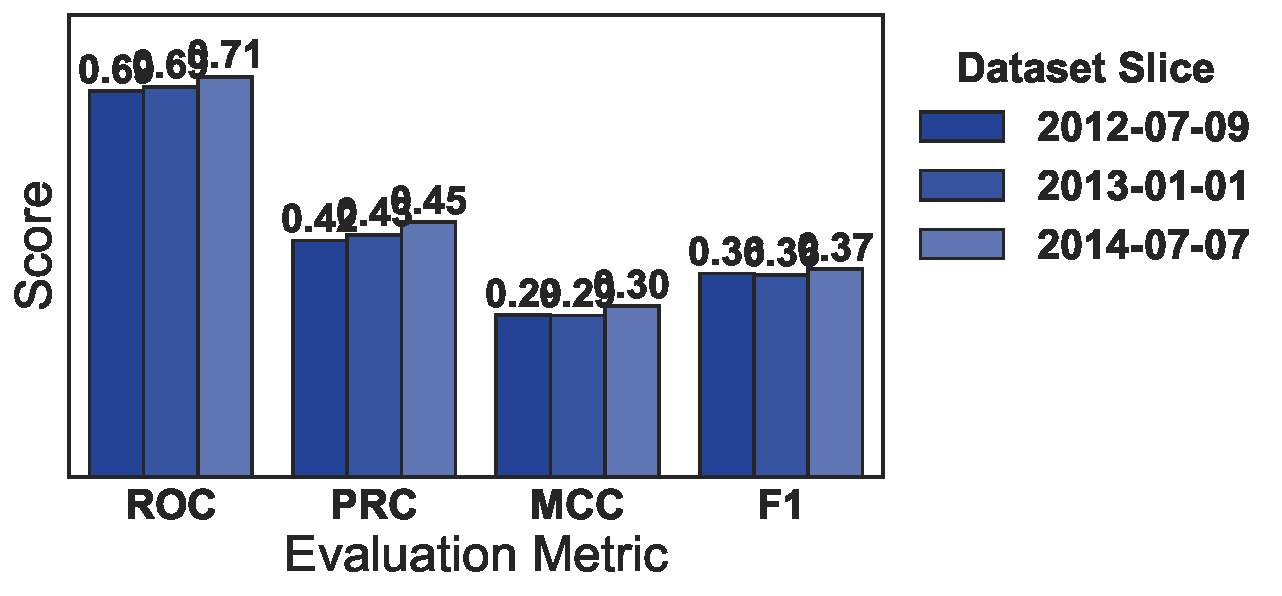
\includegraphics[width=\textwidth]{../figures/evaluation/performance_slice}
    \caption[Performance variation by slice date]{Performance variation by slice date.}
    \label{fig:evaluation:performance_slice}
\end{figure}

\begin{figure}[!htb]
    \centering
    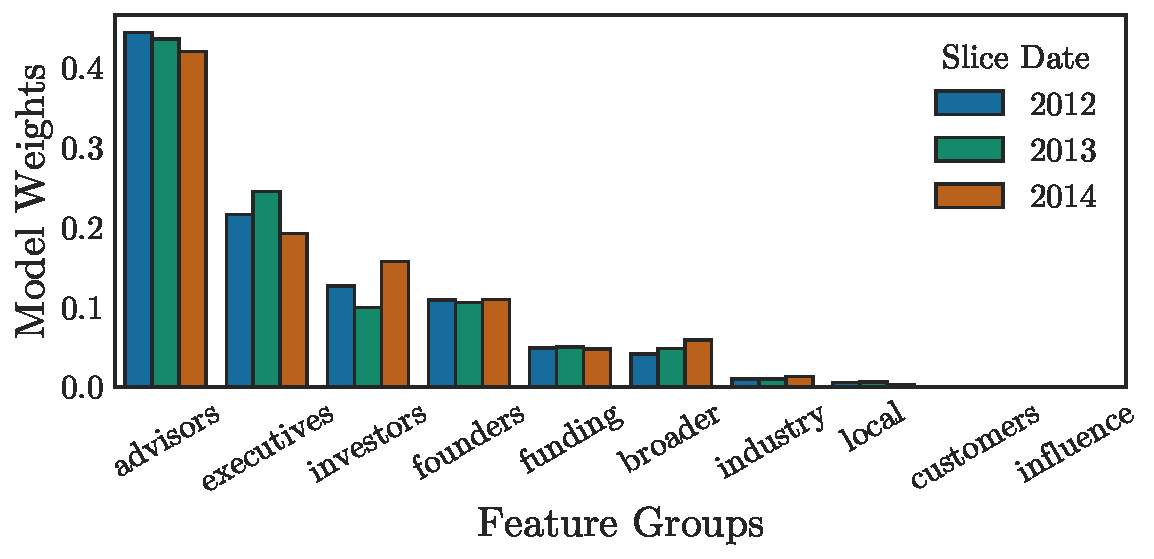
\includegraphics[width=\textwidth]{../figures/evaluation/features_slice}
    \caption[Feature weight variation by slice date]{Feature weight variation by slice date.}
    \label{fig:evaluation:features_slice}
\end{figure}

\section{Predictive Power}

The system must be consistently accurate at identifying a variety of high-potential investment candidates. We evaluated the systems' predictive power based on its ability to predict over different forecast windows (e.g. 2-4 years), for target companies at different developmental stages (e.g. Seed, Series A etc.), and for different target outcomes (e.g. predicting additional funding rounds, being acquired, having an \gls{ipo}, or some combination thereof).

\subsection{Forecast Windows}

A forecast window is the period of time between when a prediction is made and when that prediction is evaluated (i.e. a prediction made in 2014 on whether a company would exit by 2017 is a forecast window of 3 years.) The \gls{vc} industry raises funds with fixed investment horizons (3--8 years), so time to payback is a key component of \gls{vc} investment decision-making and portfolio management. It is important we understand how the models and predictions produced by a \gls{vc} investment screening system varies with respect to the length of these forecast windows.

Figure~\ref{fig:evaluation:performance_window} shows model performance across a range of metrics, grouped by forecast window. We observe little difference in Area under the \gls{roc} curve across the forecast windows. However, across all three other metrics, there is a positive relationship between length of forecast window and model performance. The F1 Score shows the greatest improvement in performance over time (52.7\%), compared to Area under the \gls{pr} curve (34.1\%) and \gls{mcc} (11.6\%).

\begin{figure}[!htb]
    \centering
    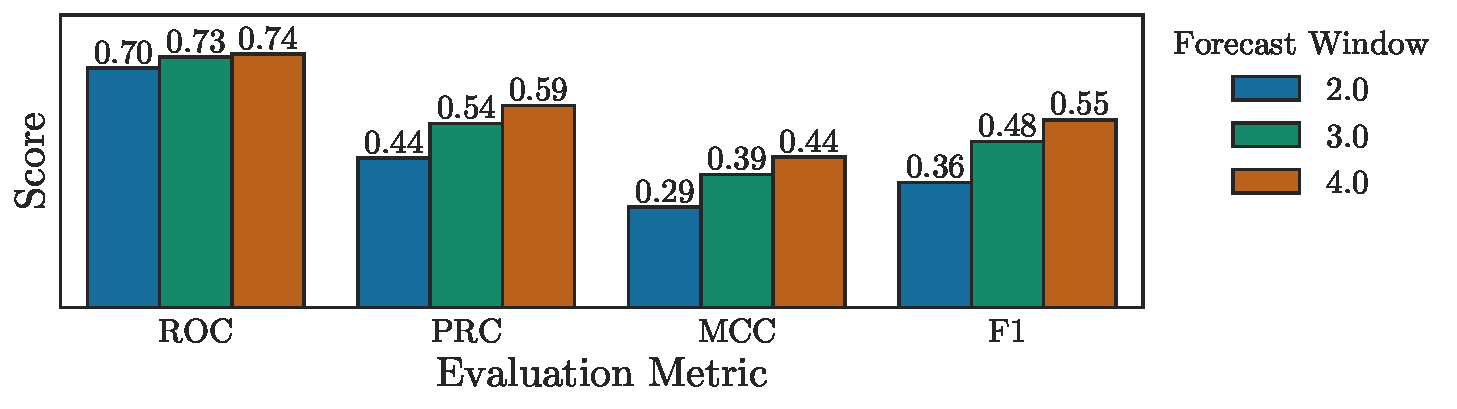
\includegraphics[width=\textwidth]{../figures/evaluation/performance_window}
    \caption[Performance by forecast window]{Performance by forecast window.}
    \label{fig:evaluation:performance_window}
\end{figure}

Figure~\ref{fig:evaluation:features_window} shows the standardised weights of features grouped using the conceptual framework proposed earlier in this paper, grouped by forecast window. First, we discuss the baseline distribution and then examine the variation in weightings with respect to forecast window. Advisors are the best predictor of startup investment success. Executives and founders are also important factors, and round out measures of human capital. The quality of investors that invest in a startup (assessed by their prior investments) is found to be more important than the quantum of investment raised by a startup. Local economy and industry factors are weak predictors, as are customers and social influence (in this case measured through participation at events). There is little difference between the weightings of each feature group with respect to forecast window. However, there are a few trends to point out: the importance of advisors increases over time, and the importance of executives and the broader economy decreases over time.

\begin{figure}[!htb]
    \centering
    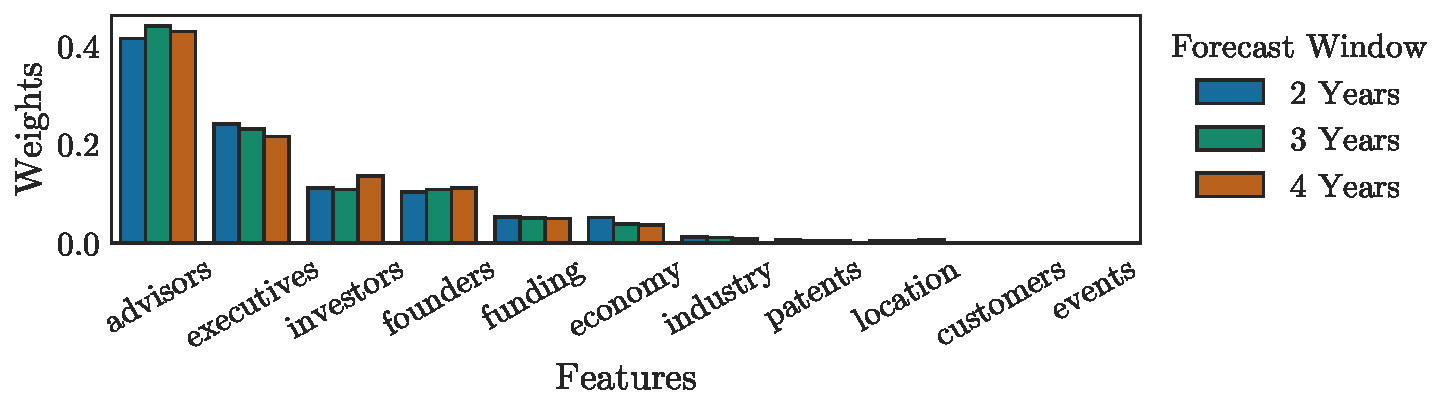
\includegraphics[width=\textwidth]{../figures/evaluation/features_window}
    \caption[Feature weights by forecast window]{Feature weights by forecast window.}
    \label{fig:evaluation:features_window}
\end{figure}

\subsection{Development Stage}

Startups can be classified into developmental stages by virtue of their external funding milestones. These milestones not only signal a change in the resources available to a startup, but also their functions and objectives, and in turn the type of investors that are interested in them as investment opportunities. In Chapter~\ref{chap:design} we mapped the companies in our dataset to their developmental stages. In the following section, we evaluated how the system models and predicts the outcomes of companies at different developmental stages.

Figure~\ref{fig:evaluation:performance_stage} shows F1 Scores grouped by developmental stage and fit method. First, we exmaine the baseline distribution and then the variation in performance by fit method. Model performance has a positive relationship with developmental stage. The only deviation from this relationship is for Series D+. To understand this discrepancy better, we split the datasets into their developmental stages and fit the model onto each of these sub-datasets individually. This results in a broad performance improvement. This method has the least impact on Pre-Seed and the greatest impact on Series D+ companies.

\begin{figure}[!htb]
    \centering
    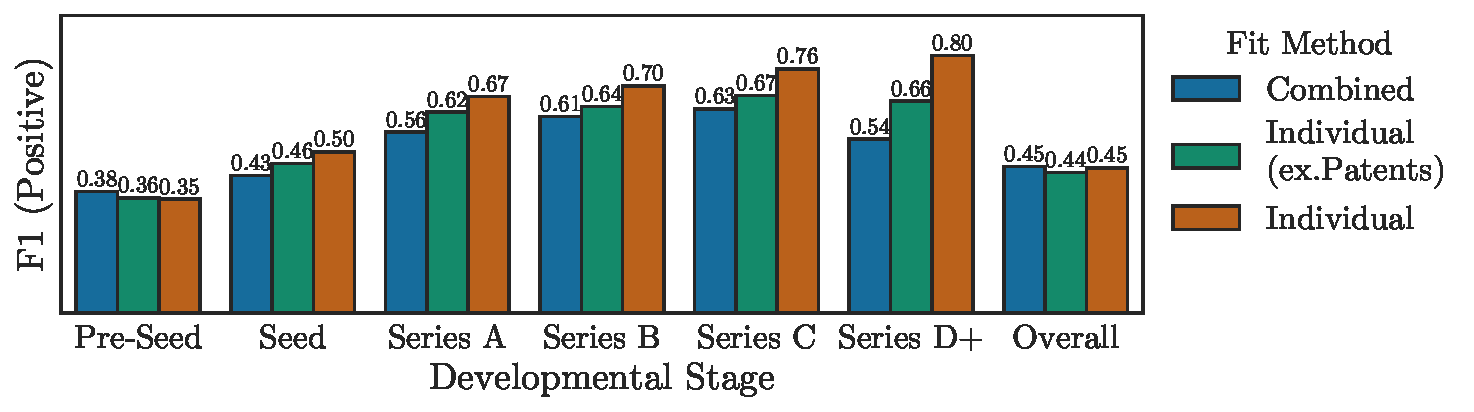
\includegraphics[width=\textwidth]{../figures/evaluation/performance_stage}
    \caption[Performance by developmental stage]{Performance by developmental stage.}
    \label{fig:evaluation:performance_stage}
\end{figure}

Figure~\ref{fig:evaluation:features_stage} shows the standardised weights of features, grouped by developmental stage. While a similar trend to Figure~\ref{fig:evaluation:features_window} is observed, there is more varation in weights than was observed when grouped by forecast window. Advisors are more important to earlier stage companies than late stage companies, investor track record and reputation becomes important as companies approach an exit (Series D+), executive and founder experience are important in pre-seed companies, as is broader economic outlook.

\begin{figure}[!htb]
    \centering
    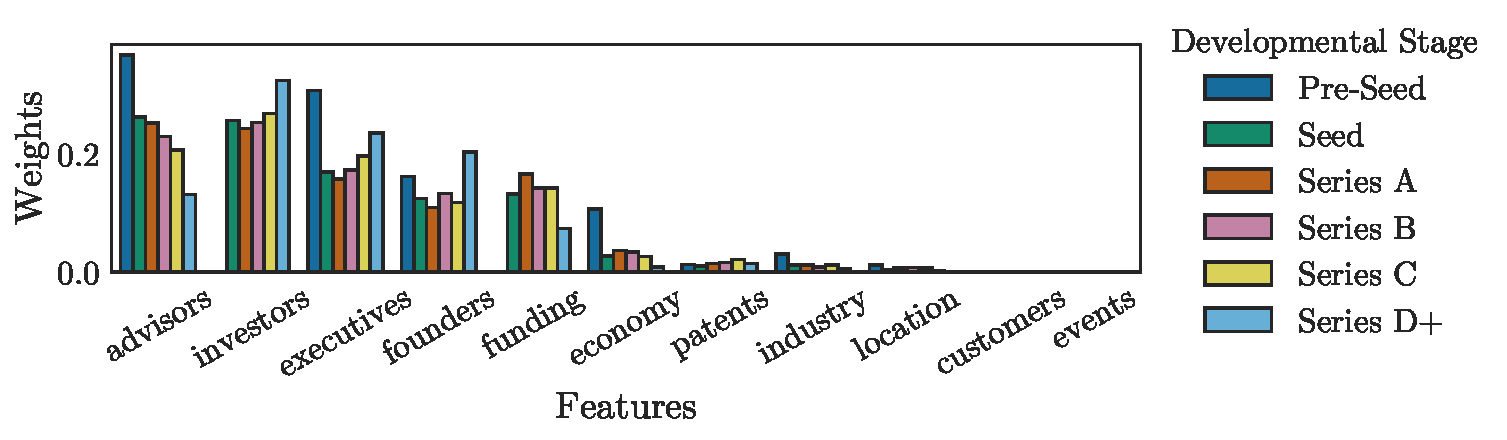
\includegraphics[width=\textwidth]{../figures/evaluation/features_stage}
    \caption[Feature weights by developmental stage]{Feature weights by developmental stage.}
    \label{fig:evaluation:features_stage}
\end{figure}

\subsection{Target Outcomes}

Ultimately, \gls{vc} firms seek rare investments that will return their invested funds many times over within an investment horizon of their fund (3-8 years). Funds are only returned to \gls{vc} investors when startups have liquidity events (\gls{ipo}, Acquisition). However, recently, many companies that are considered successful are delaying their liquidity events and seeking later-stage private funding (e.g. Uber). In this case, whether a company has raised additional funding rounds may be used as a proxy for investment success. Unless otherwise specified, we performed our previous analyses against our base target outcome, Extra Stage (i.e. whether a company raises an additional funding round, is aquired or has an \gls{ipo}). In the following section, we explore whether the component outcomes (e.g. predicting \gls{ipo}s) has an affect on our system's predictive power.

Figure~\ref{fig:evaluation:performance_stage} shows F1 Scores grouped by target outcome and forecast window. First, we examine the baseline distribution and then the variation in performance by forecast window. Our model is most accurate at predicting extra funding rounds and worst at predicting \gls{ipo}s. As we observed in Figure~\ref{fig:evaluation:performance_window}, there is a positive relationship between length of forecast window and model performance. This relationship has a similar magnitude across all target outcomes except for \gls{ipo}s which improve much more when the forecast window is increased from 2 to 3 years.

\begin{figure}[!htb]
    \centering
    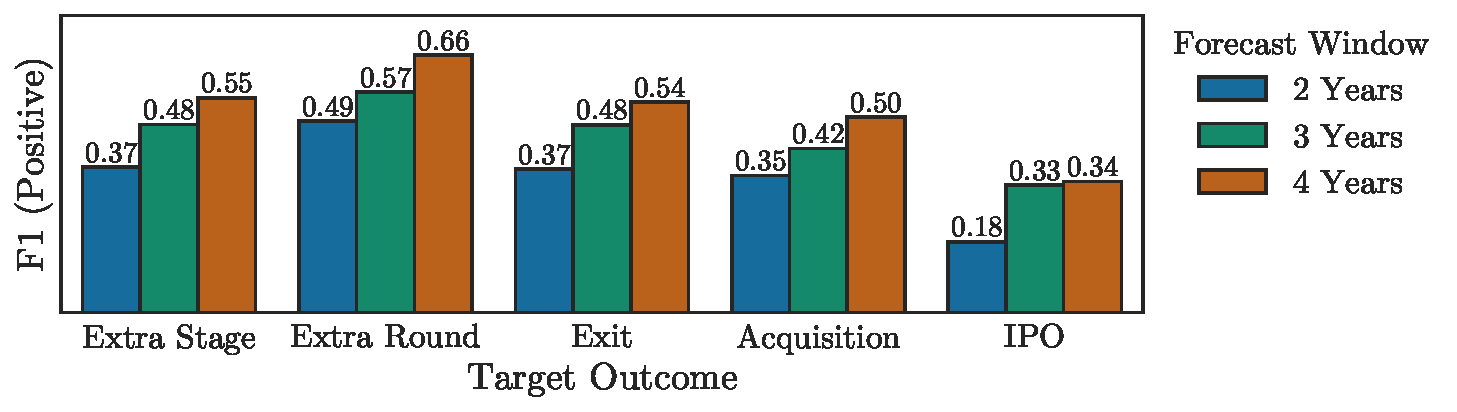
\includegraphics[width=\textwidth]{../figures/evaluation/performance_outcome}
    \caption[Performance by target outcome]{Performance by target outcome.}
    \label{fig:evaluation:f1_predictive_outcome}
\end{figure}

Figure~\ref{fig:evaluation:features_outcome} shows the standardised feature weight distribution, grouped by target outcome. Models of target outcomes produce considerable variance in feature weights. Exit and Acquisition have similar feature weights. Investors, Executives and Founders are key features for Exits and Acquisitions. In comparison, \gls{ipo}s have more weighting towards Funding, Advisors and the Broader Economy. Extra Round is most strongly related to Investors and Funding and Extra Stage is most strongly related to Advisors.

\begin{figure}[!htb]
    \centering
    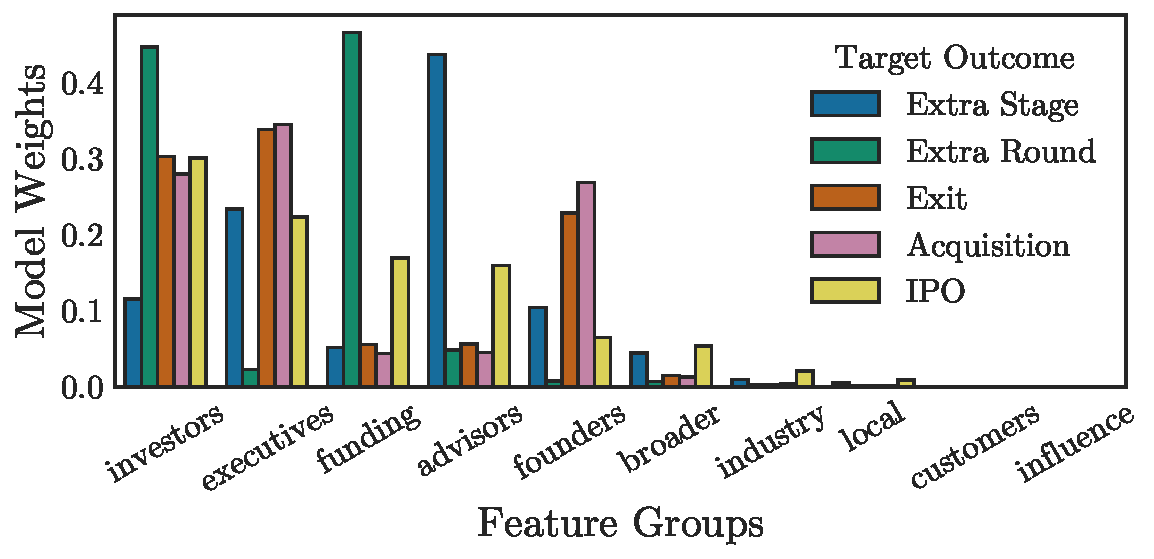
\includegraphics[width=\textwidth]{../figures/evaluation/features_outcome}
    \caption[Feature weights by target outcome]{Feature weights by target outcome.}
    \label{fig:evaluation:features_outcome}
\end{figure}

 \ifcsdef{mainfile}{}{\printbibliography}
\end{document}

